\chapter{DG CCSN}

\section{Scope and goal}

In general, I want to have a psuedo-toy simulation of a CCSN that uses DG. To constrain myself further, for simplification I will make it fully Newtonian(no GR or SR) but to add challenge I enforce positivity and well-balanced.

\section{Mathematical Model}

Rather than writing down everything, in general the math starts with the Compressible Euler, adds Polytropic steady-states and Lane-Emden equation to the hydrostatic equilibrium equation. Finally, add boundary conditions in order to enforce energy conservation.

\section{General DG}

First one creates a mesh of the given space to calculate the projection martrix.

DG projects a PDE onto a functional space of polynomials using the projection matrix. Compute the fluxes of the fluid, then fluxes of energy. Then combine this all together for the residual.

Finally, time step with choosen model.

\section{My DG}

Essentially what I have talked about with the equations I use. For the sake of brevity the link to the paper that has this all writen out is \href{https://www.sciencedirect.com/science/article/pii/S0021999126001579}{here}.

One thing I will add is a flow chart for my code


\tikzstyle{startstop} = [
    rectangle, rounded corners,
    minimum width=3cm, minimum height=1cm,
    text centered, draw=black
]
\tikzstyle{process} = [
    rectangle,
    minimum width=3cm, minimum height=1cm,
    text centered, draw=black
]
\tikzstyle{arrow} = [thick,->,>=stealth]



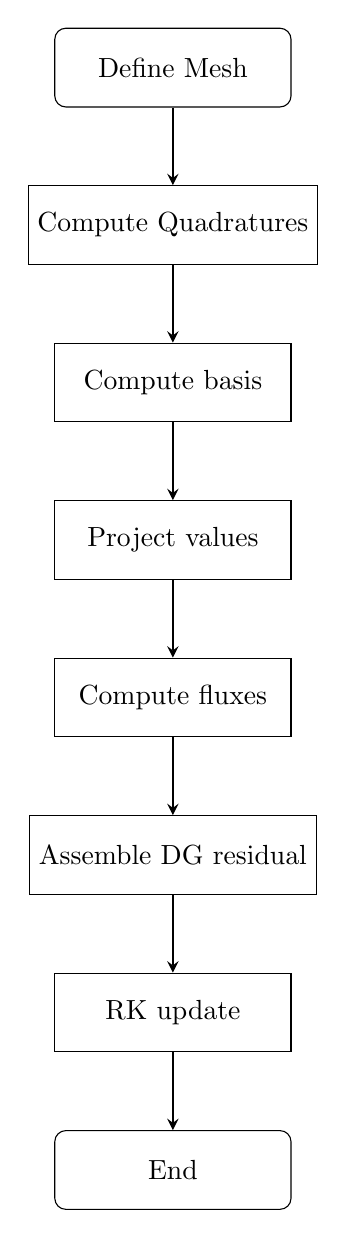
\begin{tikzpicture}[node distance=2cm]
    \node (start) [startstop] {Define Mesh};
    \node (step1) [process, below of=start] {Compute Quadratures};
    \node (step2) [process, below of=step1] {Compute basis};
    \node (step3) [process, below of=step2] {Project values};
    \node (step4) [process, below of=step3] {Compute fluxes};
    \node (step5) [process, below of=step4] {Assemble DG residual};
    \node (step6) [process, below of=step5] {RK update};
    \node (stop) [startstop, below of=step6] {End};

    \draw [arrow] (start) -- (step1);
    \draw [arrow] (step1) -- (step2);
    \draw [arrow] (step2) -- (step3);
    \draw [arrow] (step3) -- (step4);
    \draw [arrow] (step4) -- (step5);
    \draw [arrow] (step5) -- (step6);
    \draw [arrow] (step6) -- (stop);
\end{tikzpicture}

\subsection{AI overview}

Admittedly, much of this code is written by AI, I had it create documentation which I have here.


\section{General Notes}

Running the algorithm is very slow, far slower than anticipated, taking in total n hours to run the solution for first order polynomial, 16 x 16 x 16, 3rd order Runge-Kutta, and Newtonian iteration.


\section{Results}
